%%%%%%%%%%%%%%%%%%%%%%%%%%%%%%%%%%%%%%%%%%%%%%%%%%%%%%%%%%%%%%%%%%%%%%%%%%%%%%%%%%
\begin{frame}[fragile]\frametitle{}
\begin{center}
{\Large Introduction to Indian Civilization}
\end{center}
\end{frame}

%%%%%%%%%%%%%%%%%%%%%%%%%%%%%%%%%%%%%%%%%%%%%%%%%%%%%%%%%%%%%%%%%%%%%%%%%%%%%%%%%%
\begin{frame}[fragile]\frametitle{Introduction}
\begin{columns}
\begin{column}{0.5\textwidth}
\begin{itemize}
\item Indus Valley Civilization (c. 3300-1300 BCE)
\item Emerged along the Indus River in modern-day Pakistan and India
\item Developed sophisticated urban centers, sanitation, and trade networks
\item Evidence of advanced mathematics, astronomy, and urban planning
\item Decline likely due to climate change and environmental degradation
\end{itemize}
\end{column}
\begin{column}{0.5\textwidth}
\begin{figure}
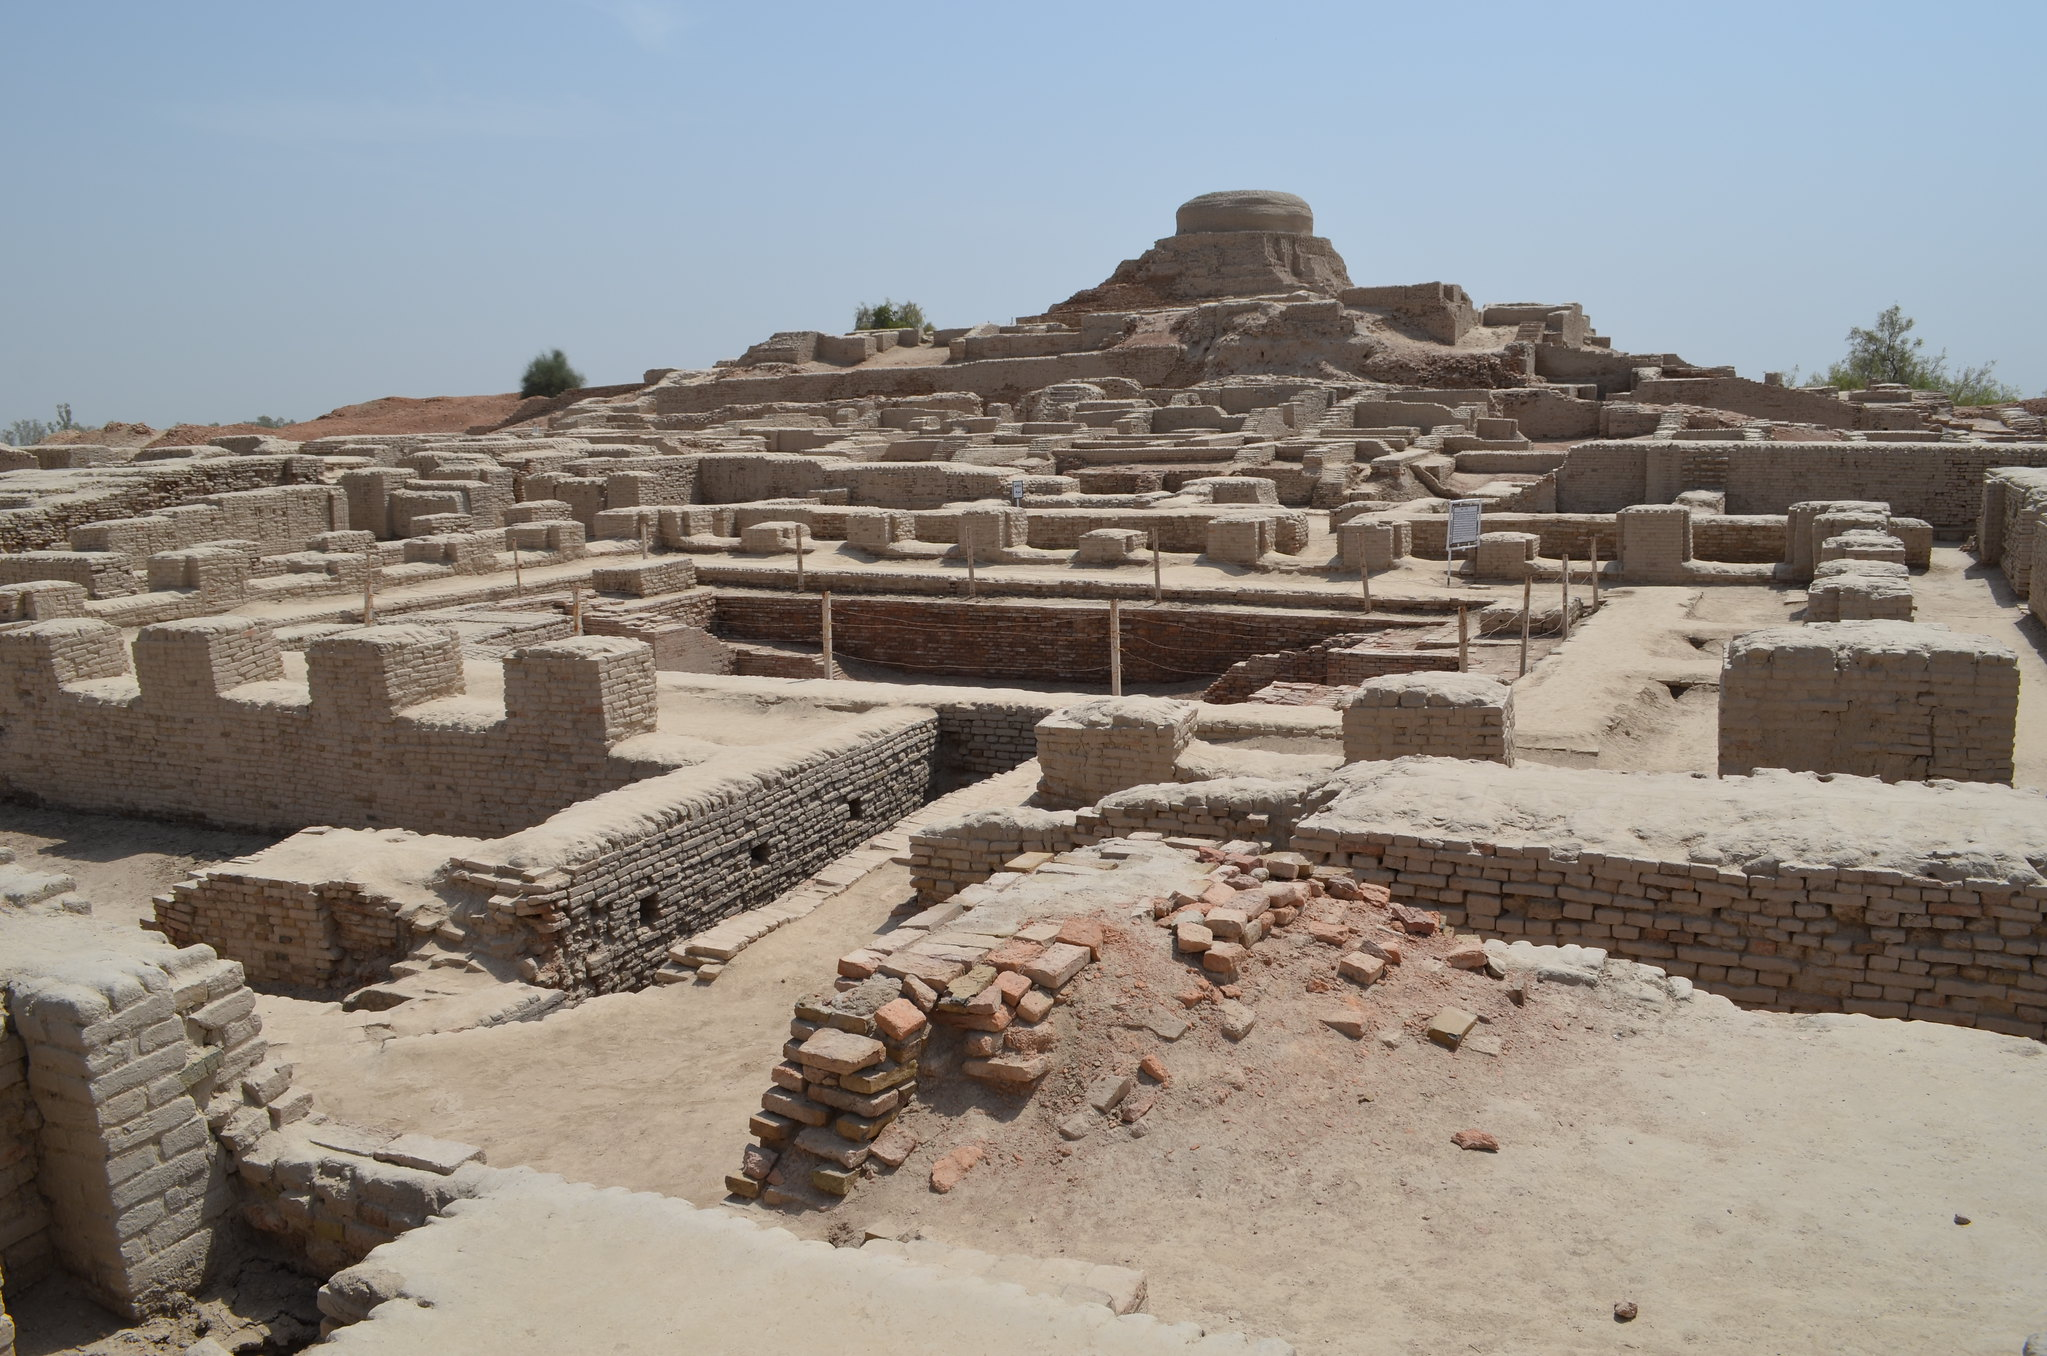
\includegraphics[width=\linewidth]{indus-valley-civilization.jpg}
\caption{Ruins of Mohenjo-daro, a major city of the Indus Valley Civilization - World History Encyclopedia}
\end{figure}
\end{column}
\end{columns}
\end{frame}